\documentclass[11pt]{article}

\usepackage{amsmath}
\usepackage{amssymb}
\usepackage{booktabs}
\usepackage[margin=1in]{geometry}
\usepackage{hyperref}
\usepackage{listings}
\usepackage{xcolor}
\usepackage{tikz}
\usetikzlibrary{arrows.meta,positioning}
\hypersetup{colorlinks=true,linkcolor=blue,citecolor=blue,urlcolor=blue}

% Long \texttt tokens (namespaced MATLAB calls) do not hyphenate; give the
% paragraph builder room rather than leaving overfull boxes.
\setlength{\emergencystretch}{4em}
\hbadness=10000
\tolerance=2000

\newcommand{\code}[1]{\texttt{#1}}
\newcommand{\pkg}[1]{\texttt{+#1}}

\lstset{
  basicstyle=\ttfamily\footnotesize,
  columns=fullflexible,
  keepspaces=true,
  breaklines=true,
  frame=single,
  framesep=3pt,
  rulecolor=\color{gray!50},
  backgroundcolor=\color{gray!6},
  showstringspaces=false,
  aboveskip=5pt,
  belowskip=5pt
}

% Tables in this document are reference material, not prose: set them a size
% down and tighten the row spacing so a wide one stays on one page.
\usepackage{etoolbox}
\AtBeginEnvironment{tabular}{\small}
\renewcommand{\arraystretch}{1.05}

\title{Software Design\\
       \large Architecture and data flow of the \code{missiles/} trajectory library}
\author{Coorbital, Inc.}
\date{7 August 2026}

\begin{document}
\maketitle

\begin{abstract}
This is the software-design companion to \code{docs/hgv\_dynamics\_note.tex}.
That note derives the mathematics; this one describes the \emph{structure} ---
where the module boundaries fall and why, how a trajectory moves through the
code from a user's parameter block to a rendered movie, which design decisions
were forced by the language or the solver and which were chosen, what the
alternatives were, and where a choice was later proved right or wrong by
measurement. It is not a function reference: \code{docs/README.md} already
lists what each file does and is the authority on delivered behaviour.

Every structural claim below was checked against the committed source, and the
measurements were re-run for this document rather than carried over. The full
verification record is Section~\ref{sec:verify}. Where this document and the
narrative in \code{docs/README.md} or \code{docs/DESIGN.md} disagree on a
count or a number, the discrepancy is named at the point it occurs.
\end{abstract}

\tableofcontents

%=====================================================================
\section{Scope and the document set}

\subsection{What this document is for}

The library has three prose documents and two \LaTeX{} notes, and they divide
along a deliberate line.

\begin{center}
\begin{tabular}{lll}
\toprule
Document & Answers & Authority for \\
\midrule
\code{DESIGN.md}                & what was \emph{intended}     & the pre-implementation spec, unedited \\
\code{README.md}                & what each file \emph{does}   & delivered behaviour \\
\code{LESSONS\_LEARNED.md}      & what \emph{broke}            & the running log \\
\code{TODO.md}                  & what is \emph{open}          & the open-items list \\
\code{hgv\_dynamics\_note.tex}  & the \emph{mathematics}       & the equations and the closed forms \\
\textbf{this file}              & the \emph{structure}         & boundaries, data flow, rationale \\
\bottomrule
\end{tabular}
\end{center}

No equation of motion is derived here. Where the design turns on a piece of
mathematics --- the two-component gravity signature, the seven-state lift, the
one-sided event directions --- the reason for the \emph{interface} is given and
the derivation is cited to the dynamics note by section.

\paragraph{Why this file appears two milestones late.} \code{DESIGN.md} \S8
says the two \LaTeX{} notes are ``written after the first milestone, when the
interfaces have survived contact with working code''; the deferral is then
recorded twice, in \S10.1 and \S11.1. It was correct. Several of the design
decisions explained below did not exist when the first milestone shipped, and
one of them --- the promised \code{+util/stateConvert.m} --- was predicted,
then abandoned, then replaced by something structurally different. A
software-design document written in August's first week would have described a
mapping layer that will never be built.

\subsection{The three constraints that shaped everything}

Three requirements, all present before any code, account for most of the
architecture, and it is worth naming them before the packages.

\begin{description}
\item[Throughput.] \code{DESIGN.md} \S1 quotes the capability target:
``Computationally Efficient Open-loop Controllers Create Multiple
Trajectories/Second.'' Prescribed-control simulation comes first and
optimisation second \emph{because} of this, and it is why the entry scripts
carry a programmatic override path (Section~\ref{sec:entry}) rather than only
an editable block. A propagation here measures about $0.15~\mathrm{s}$, which
is what makes a twelve-propagation bisection a two-second script.

\item[Fidelity as a one-line change.] The library ships the crudest usable
model in every family, on purpose, because those are the models with closed-form
solutions to validate against. It must be possible to replace any of them
without editing the equations of motion, the integrator, the guidance, the
events or the plotting. This is Section~\ref{sec:inject}, and it is the single
most consequential decision in the tree.

\item[Analytic validation first.] A spherical, non-rotating Earth with an
exponential atmosphere has closed-form solutions; an oblate rotating Earth with
tabulated aerodynamics has none. The build order runs simple-first so that
every increment lands behind a check that already works. The testing discipline
that grew out of this (Section~\ref{sec:test}) is the most distinctive thing in
the repository.
\end{description}

%=====================================================================
\section{Architecture and the dependency graph}
\label{sec:arch}

\subsection{The one-package rule}

Everything reusable lives in a single \code{+coorbital} package with eight
subpackages. The vehicle folders \code{HGV/} and \code{BM/} hold
\textbf{only} parameter files and entry scripts and contain no physics
whatever. That rule is what makes the vehicle folders cheap: adding
\code{ICBM/} costs two files and no library change, and \code{tests/run\_tests}
already looks for it on the path and skips it silently when it is absent.

Counted against the source on 7 August 2026: 53 \code{.m} files, of which 26
are under \code{+coorbital} (23 public library functions plus three
package-private helpers in \code{+viz/private}), 21 under \code{tests/}
(\code{run\_tests.m} and twenty \code{test\_*.m}), and six across \code{HGV/}
and \code{BM/}. Note that \code{README.md}'s conventions section still says
``39 \code{.m} files''; \code{TODO.md} already records that as a stale count
rather than a violation.

\subsection{What each package owns}

\begin{center}
\begin{tabular}{llp{7.2cm}}
\toprule
Package & Kind & Owns \\
\midrule
\pkg{util}  & foundation   & the constants (\code{missileConst}), the two vehicle and one booster parameter sets, spherical-trigonometry helpers (\code{greatCircle}, \code{greatCircleBearing}), and the black-box scalar solver \code{rangeSolve} \\
\pkg{atmos} & model        & density, pressure, temperature, sound speed from altitude \\
\pkg{grav}  & model        & radial and latitudinal gravitational acceleration \\
\pkg{aero}  & model        & lift and drag coefficients \\
\pkg{eom}   & physics      & the six-state unpowered and seven-state powered right-hand sides, plus \code{massConstant}, the adapter between them \\
\pkg{guide} & control      & control-schedule evaluation: open-loop \code{prescribed} and state-reading \code{pitchProgram} \\
\pkg{prop}  & driver \emph{and} model & \code{phaseRun} and the three ODE events (propagator); \code{constThrust} (propulsion) \\
\pkg{viz}   & presentation & four figure functions and three package-private helpers \\
\bottomrule
\end{tabular}
\end{center}

\paragraph{The one bad name, kept deliberately.} \pkg{prop} holds both the
\emph{propagator} and \emph{propulsion}. Two meanings of one abbreviation in
one namespace is a genuine wart. It was not worth a rename because propulsion
models are identified by their \emph{signature},
\code{[T,mdot] = f(t,P,veh)}, not by their package, and the rename would have
touched every entry script and every test for a cosmetic gain.
\code{README.md} says so explicitly rather than leaving a reader to wonder
whether it was noticed.

\subsection{The dependency graph}

Dependencies were read off the source by resolving every
\code{coorbital.*} call site. The graph is a DAG with \pkg{util} at the bottom
and \pkg{viz} hanging off to the side.

\begin{center}
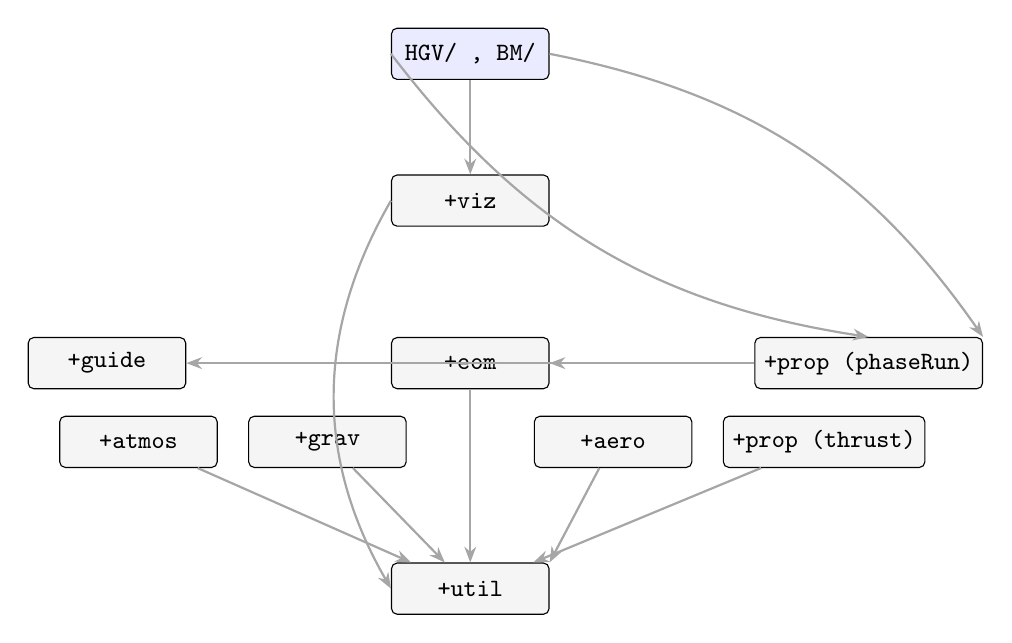
\begin{tikzpicture}[
   >={Stealth[length=2mm]},
   node distance=8mm and 10mm,
   box/.style={draw,rounded corners=2pt,minimum height=6.5mm,minimum width=20mm,
               font=\small\ttfamily,fill=gray!8},
   ent/.style={box,fill=blue!8},
   dep/.style={->,gray!70,thick}
  ]
  \node[box] (util)  {+util};
  \node[box,above left=12mm and 22mm of util]  (atmos) {+atmos};
  \node[box,above left=12mm and -2mm of util]  (grav)  {+grav};
  \node[box,above right=12mm and -2mm of util] (aero)  {+aero};
  \node[box,above right=12mm and 22mm of util] (propm) {+prop (thrust)};

  \node[box,above=22mm of util] (eom) {+eom};
  \node[box,left=26mm of eom]   (guide) {+guide};
  \node[box,right=26mm of eom]  (run)  {+prop (phaseRun)};
  \node[box,above=14mm of eom]  (viz)  {+viz};
  \node[ent,above=12mm of viz]  (scr)  {HGV/ , BM/};

  \draw[dep] (atmos) -- (util);
  \draw[dep] (grav)  -- (util);
  \draw[dep] (propm) -- (util);
  \draw[dep] (aero)  -- (util.north east);
  \draw[dep] (eom)   -- (util);
  \draw[dep] (viz.west)  to[bend right=30] (util.west);
  \draw[dep] (run)   -- (eom);
  \draw[dep] (run)   -- (guide);
  \draw[dep] (scr)   -- (viz);
  \draw[dep] (scr.west) to[bend right=22] (run.north);
  \draw[dep] (scr.east) to[bend left=22]  (run.north east);
\end{tikzpicture}
\end{center}

Read as a table, with the edges that matter and the edges that are notable by
their \emph{absence}:

\begin{center}
\begin{tabular}{lll}
\toprule
Package & Depends on & Does \textbf{not} depend on \\
\midrule
\pkg{util}   & nothing                       & everything else \\
\pkg{atmos}  & \pkg{util}                    & \pkg{eom}, \pkg{grav}, \pkg{aero} \\
\pkg{grav}   & \pkg{util}                    & \pkg{eom}, \pkg{atmos} \\
\pkg{aero}   & \pkg{util} (self-demo only)   & \pkg{eom}, \pkg{atmos} \\
\pkg{prop} (thrust) & \pkg{util}, \pkg{atmos} (self-demo only) & \pkg{eom}, \pkg{grav} \\
\pkg{eom}    & \pkg{util}; \emph{handles} into the four model families & any named model \\
\pkg{guide}  & nothing                       & \pkg{eom}, \pkg{util} \\
\pkg{prop} (\code{phaseRun}) & \pkg{eom}, \pkg{guide} \emph{through handles} & the models \\
\pkg{viz}    & \pkg{util}                    & \pkg{eom}, \pkg{prop}, the models \\
\code{HGV/}, \code{BM/} & everything          & --- \\
\bottomrule
\end{tabular}
\end{center}

Four properties of this graph are load-bearing.

\begin{enumerate}
\item \textbf{\pkg{util} is a leaf.} \code{missileConst} imports nothing. That
is what lets it be the single source of truth: every other package can reach it
without a cycle, and a constant therefore has exactly one home. The alternative
considered and rejected was wrapping pumpkyn's \code{getConst}, which has no
\code{muE}, no Earth radius, and two fields known to be wrong. Wrapping it
would have made the library's foundation depend on a struct that cannot supply
its two most important members.

\item \textbf{The four model packages do not know about each other.} There is
no edge from \pkg{prop} to \pkg{atmos} in the shipped code path --- ambient
pressure is \emph{handed} to the propulsion model rather than looked up by it
(Section~\ref{sec:pressure}), so swapping the atmosphere does not touch
propulsion. The only \code{coorbital.atmos} reference inside
\code{constThrust.m} is in its \code{nargin == 0} self-demo, which needs a
sea-level pressure to print.

\item \textbf{\pkg{eom} names no model.} It reaches all four families through
function handles on an \code{env} struct. This is Section~\ref{sec:inject}.

\item \textbf{\pkg{viz} is a sink.} It depends only on \pkg{util}, for the
Earth radius, and nothing depends on it. That is what allows the claim below.
\end{enumerate}

\subsection{\pkg{viz} reads trajectories and never writes them}
\label{sec:vizreadonly}

Every figure function takes the same \code{(traj,veh,env,opts)} argument list
and returns a graphics handle or a movie record. None writes to \code{traj}.
That is easy to assert and worth measuring, because it is the property that
lets a reader trust that a summary printed above a figure call is the same
number it would have been with figures off.

\textbf{Measured for this document, 7 August 2026.} Each entry script was run
twice --- once with \code{showPlots} true, once false --- with the printed
summary captured by \code{evalc} and the returned trajectory compared with
\code{isequaln}:

\begin{center}
\begin{tabular}{lrrl}
\toprule
Script & Summary lines & Lines differing & \code{isequaln(traj)} \\
\midrule
\code{run\_glide}       &  42 & 0 & true \\
\code{run\_ballistic}   & 105 & 0 & true \\
\code{run\_boost\_glide}& 127 & 0 & true \\
\code{run\_target}      & 149 & 0 & true \\
\bottomrule
\end{tabular}
\end{center}

Zero differing lines across 423 lines of summary, and the returned trajectory
is \code{isequaln}-identical in all four cases. (The three chain scripts alone
account for 274 of those lines.) The figures cannot move a number, and this is
now a measurement rather than a convention.

%=====================================================================
\section{Model injection}
\label{sec:inject}

\subsection{The mechanism}

The equations of motion never name a model. They call function handles carried
on an environment struct:

\begin{lstlisting}
env.atmos  = @coorbital.atmos.expAtmos;    % [rho,P,T,a] = f(h)
env.grav   = @coorbital.grav.sphereGrav;   % [gr,gLat]   = f(r,lat)
env.aero   = @coorbital.aero.constLD;      % [CL,CD]     = f(alpha,mach,veh)
env.prop   = @coorbital.prop.constThrust;  % [T,mdot]    = f(t,P,veh)   powered only
env.omegaE = 0;                            % scalar, not a handle
\end{lstlisting}

Inside \code{glide3DOF} the corresponding three lines are literally:

\begin{lstlisting}
   [rho,~,~,aSnd] = env.atmos(h);
        [gr,gLat] = env.grav(r,lat);
          [CL,CD] = env.aero(alpha,V./aSnd,veh);
\end{lstlisting}

with \code{boost3DOF} adding \code{[T,mdot] = env.prop(t,P,veh);}. There is no
\code{switch}, no registry, no model name anywhere in either file.

\subsection{Why handles and not a switch, a class, or a subclassed model}

Three alternatives were available and each is worse for this library.

\begin{description}
\item[A \code{switch} on a model-name string.] Every new model then edits the
equations of motion --- the one file whose correctness the whole suite rests
on --- and every edit is an opportunity to break a shared term.

\item[An abstract class per family with concrete subclasses.] MATLAB's
\code{classdef} dispatch is measurably slower than a function-handle call in a
tight derivative loop, and a derivative is evaluated hundreds of thousands of
times across a chain. The throughput requirement in \code{DESIGN.md} \S1 is
what rules this out; the boilerplate cost of one \code{classdef} per model in a
library whose smallest model is 15 lines of executable code is the second
reason.

\item[Passing the models positionally.] \code{f(t,x,u,veh,atmosFn,gravFn,\dots)}
grows the signature every time a family is added --- and a family \emph{was}
added: propulsion arrived a milestone after the other three. The \code{env}
struct absorbed it with no signature change anywhere.
\end{description}

The handle-on-a-struct form pays for itself precisely because the fourth
family arrived late. \code{env.prop} is read only by \code{boost3DOF}; an
unpowered chain omits it entirely and \code{glide3DOF} ignores it if present.
No file changed to make that work.

\subsection{Why gravity returns two components when the shipped one is zero}

\code{sphereGrav} returns \code{gLat = zeros(size(r))} --- identically zero, at
every state, forever. A scalar interface \code{g = f(r)} would be simpler and
would produce bit-identical trajectories today.

It was rejected because \textbf{$J_2$ has a latitudinal acceleration that a
single ``local up'' scalar cannot represent}. Committing to a scalar now would
mean that the day \code{j2Grav} arrives, the signature changes and
\emph{every call site in \code{glide3DOF} and \code{boost3DOF} has to be
rewritten} --- in three separate equations, $\dot V$, $\dot\gamma$ and
$\dot\psi$, each needing a new projection of $g_\phi$ onto the velocity frame,
under time pressure, with no test that exercises the new terms because they did
not exist an hour earlier. The projections are derived in the dynamics note,
\S3.2.

So the second output exists from the first commit and the projection terms are
already written into both EOM files, multiplying out to zero under spherical
gravity. \code{README.md} records the injection test that proves the plumbing
is live: replacing \code{env.grav} with a handle returning
$g_\phi = 0.01~\mathrm{m/s^2}$, with no edit to \code{glide3DOF}, changes
$\dot\psi$ by $-1.667\times10^{-6}~\mathrm{rad/s}$, exactly
$-g_\phi\sin\psi/(V\cos\gamma)$.

\paragraph{The cost, stated plainly.} Those three $g_\phi$ terms are dead code
under every shipped configuration and are unexercised by the twenty tests. The
dynamics note verified them separately, against an independent vector
reconstruction with a synthetic $g_\phi$, and says a reviewer should treat them
as verified by that note and by nothing else in the repository. Carrying dead
code is a real cost; it was accepted because the alternative is an interface
break at the worst possible moment.

\subsection{Why the propulsion model takes pressure, not altitude}
\label{sec:pressure}

The signature is \code{[T,mdot] = f(t,P,veh)} with \code{P} in pascals. The
obvious alternative, \code{f(t,h,veh)}, was rejected for a reason that is about
coupling rather than about physics.

The back-pressure debit acts on the nozzle exit plane and is a \emph{pressure}
term, $A_e(P_e - P)$. A model handed an altitude would have to hold its own
atmosphere to recover $P$ --- and that private atmosphere would either
duplicate \code{env.atmos} or, worse, silently contradict it. Swap
\code{expAtmos} for a US-76 model and the trajectory would then be flown
through one atmosphere while the motor was debited against another, with
nothing anywhere reporting the inconsistency.

The equations of motion already have $P$ in hand --- \code{boost3DOF} unpacks
\code{[rho,P,\textasciitilde,aSnd] = env.atmos(h)} one line earlier --- so
passing it costs nothing and makes propulsion \emph{independent of which
atmosphere is installed}. Every propulsion model follows an atmosphere swap
automatically. This is the third dependency edge that the graph in
Section~\ref{sec:arch} does \emph{not} have.

\subsection{Why Earth rotation is a scalar and not a handle}

\code{env.omegaE} is a number, not a function. It is the one environment entry
that is not injectable, and correctly so: rotation is not a \emph{model} with
alternative implementations, it is a single parameter of the frame. The
Coriolis and centrifugal terms are written into both EOM files from the first
commit and gated on \code{if om \textasciitilde= 0}, so setting it to zero
recovers the non-rotating case \emph{exactly} --- the block is skipped, not
multiplied by zero. All four entry scripts expose it as the boolean
\code{earthSpin}, shipped \code{false}.

\subsection{The end-to-end test, and the defect it found}
\label{sec:injecttest}

The promise is that raising fidelity is a one-line change in an entry script.
Restating a promise is not testing it, so it was exercised: a scratch $J_2$
gravity model and a scratch throttled engine were written outside the tree,
signature-compatible with the shipped ones, and swapped in through the entry
scripts' override whitelists --- one struct field each, no library edit.

\begin{lstlisting}
[traj,info] = run_ballistic(struct('showPlots',false, ...
                                   'gravFn',@j2GravScratch, ...
                                   'propFn',@throttleScratch));
\end{lstlisting}

\textbf{Measured, 7 August 2026, on the committed library:}

\begin{center}
\begin{tabular}{lll}
\toprule
Call & Swap & Result \\
\midrule
\code{run\_glide}        & \code{gravFn}             & ran; terminal point moved $17.30~\mathrm{km}$ \\
\code{run\_ballistic}    & \code{gravFn}             & ran; range $4517.320~\mathrm{km}$ \\
\code{run\_ballistic}    & \code{gravFn}, \code{propFn} & ran; range $4588.940~\mathrm{km}$ \\
\code{run\_boost\_glide} & \code{gravFn}, \code{propFn} & ran; range $7266.004~\mathrm{km}$ \\
\bottomrule
\end{tabular}
\end{center}

\paragraph{The defect.} Before 7 August 2026, the second row \emph{aborted}.
\code{BM/run\_ballistic} carries a Keplerian cross-check: it re-propagates the
burnout state with aerodynamics off and compares against the closed-form
free-flight range of the same two-body arc, asserted at $10^{-6}$ relative,
with a message insisting that ``a disagreement is a defect, not a modelling
difference.'' That re-propagation \emph{inherited} \code{env.grav}. Select an
oblate model and the check flew a $J_2$ arc against a two-body reference and
fired on the $J_2$ signal --- which \emph{was} a modelling difference, exactly
what the assertion's own message said a failure was not.

The fix is three characters of intent and one line of code: the cross-check
pins its own gravity.

\begin{lstlisting}
        envVac      = env;
        envVac.aero = @(alphaArg,machArg,vehArg) deal(0,0);
        envVac.grav = @coorbital.grav.sphereGrav;   % <-- pinned, not inherited
      envVac.omegaE = 0;
\end{lstlisting}

The main run still flies whatever gravity the user selected; only the one
validation that has a two-body closed form to answer to is forced back to
\code{sphereGrav}, and the source comment says why at the point of the pin.

\textbf{Reproduced for this document.} The burnout state of the $J_2$ run was
propagated to impact twice, once inheriting $J_2$ and once on
\code{sphereGrav}, and compared against the same two-body closed form:

\begin{center}
\begin{tabular}{lr}
\toprule
Cross-check gravity & Relative disagreement (budget $10^{-6}$) \\
\midrule
inherited $J_2$ (pre-fix behaviour)   & $2.947\times10^{-3}$ \\
pinned \code{sphereGrav} (shipped)    & $5.207\times10^{-12}$ \\
\bottomrule
\end{tabular}
\end{center}

That is a factor of $5.7\times10^{8}$, and the upper figure sits in the
$2.9\times10^{-3}$ to $3.2\times10^{-3}$ band \code{README.md} reports for the
original measurement.

Two general points come out of it. First: \textbf{this was found by exercising
the extensibility promise, not by restating it}. Nothing in the twenty tests
touches it, because every test runs the default models. Second: the exception
is documented \emph{as} an exception, in the user block itself
(\code{run\_ballistic.m}, the \code{gravFn} comment) and in
\code{README.md}'s ``Adding a fidelity level'' section, so a reader following
the recipe meets the caveat before the failure. Both entry scripts also gate
their printed validity paragraphs on the handles actually being the defaults,
so a swapped model no longer produces the sentence ``the spherical
\code{j2Grav} carries no J2''.

%=====================================================================
\section{Data flow: one run end to end}
\label{sec:flow}

\subsection{The trajectory struct}

Everything downstream of the propagator consumes one struct, produced in one
place, at the bottom of \code{coorbital.prop.phaseRun}:

\begin{center}
\begin{tabular}{lll}
\toprule
Field & Shape & Contents \\
\midrule
\code{traj.t}        & $[N\times1]$        & cumulative time (s), strictly increasing \\
\code{traj.x}        & $[N\times n_x]$     & state; $n_x = 6$ unpowered, $7$ with a powered phase \\
\code{traj.u}        & $[N\times n_u]$     & control (rad on both angle channels), $n_u = 2$ today \\
\code{traj.phaseIdx} & $[N\times1]$        & 1-based phase label per sample \\
\code{traj.junction} & $[(P-1)\times1]$ struct & fields \code{t} (s) and \code{x} $[n_x\times1]$ \\
\bottomrule
\end{tabular}
\end{center}

$n_x$ and $n_u$ are both \emph{measured}, never assumed: $n_x$ from
\code{numel(x0)} and $n_u$ from one call to phase~1's guide before the loop.
The consequence of measuring $n_u$ that way is written into \code{phaseRun}'s
header and is a genuine interface obligation: \textbf{a stateful guide --- one
that latches, counts calls, or otherwise remembers what it has been asked ---
sees one evaluation more than the integrator makes and must tolerate it.} No
shipped guide is stateful; a future closed-loop law might be.

A single-phase run returns \code{traj.junction} as a $0\times1$ struct array,
not an empty matrix, so a consumer can \code{numel} it without a special case.

\subsection{The trace}

Take \code{HGV/run\_boost\_glide} as the representative run. Eleven steps, in
order:

\begin{enumerate}
\item \textbf{Path resolution.} \code{addpath} of the script's own folder and
of the library root, from \code{mfilename('fullpath')}, so the script runs from
any working directory once MATLAB can see the file.

\item \textbf{The user block.} A fenced \code{\%\% USER PARAMETERS:} region of
literal assignments in \emph{human} units --- degrees, kilometres, seconds ---
each with an inline comment giving its unit and its sensible range.

\item \textbf{Overrides.} If \code{opts} was supplied, each named entry is
replaced. This happens \emph{before} unit conversion, so a caller writes
degrees and kilometres exactly as the block does. An unrecognised field raises.

\item \textbf{Unit conversion.} One block, one time, converting the whole user
block to SI. A source comment marks it as the only conversion in the file, and
nothing below it works in any other unit.

\item \textbf{Validation of the block.} Cheap assertions before anything
expensive: pitch grid strictly increasing and matching its angle vector, stop
altitude below the pad, launch speed above the $1~\mathrm{m/s}$ singularity,
every horizon positive.

\item \textbf{Mass bookkeeping and the per-phase vehicles.} Liftoff, burnout
and post-separation masses are computed from the parameter structs; the glide
vehicle is chosen from the separation flag and its \code{mass} field set to the
mass actually carried. This is Section~\ref{sec:mass}.

\item \textbf{Environment assembly.} The five \code{env} fields from the
handles chosen in the block.

\item \textbf{Phase construction.} A $[1\times3]$ struct array, each element
carrying \code{eom}, \code{guide}, \code{terminate}, \code{tspan} and
\code{link}.

\item \textbf{Propagation.} One call:
\code{traj = coorbital.prop.phaseRun(ph,x0,bst,env)}. Inside, per phase:
\code{ode45} with \code{RelTol = AbsTol = 1e-10} and the phase's event
function; then the control history is rebuilt on the returned grid; then the
duplicated first sample is dropped for every phase after the first; then the
segment's time is re-referenced to the phase's own \code{tspan(1)} and offset
onto the cumulative clock; then the optional \code{link} is applied and the
junction recorded. After the loop, four \code{vertcat} calls assemble the
output.

\item \textbf{Derived quantities and the summary.} Dynamic pressure, Mach,
load factors, great-circle ranges, per-phase means, a counterfactual
propagation, a termination diagnosis per phase, and the printed block. The
same numbers go into the \code{info} output at full precision.

\item \textbf{Figures.} Three \code{coorbital.viz} calls, all read-only
(Section~\ref{sec:vizreadonly}), gated on \code{showPlots}.
\end{enumerate}

\subsection{Where the control history comes from}

\code{traj.u} is not produced by \code{ode45}. The integrator is handed a
closure that evaluates the guide internally:

\begin{lstlisting}
              odeF = @(t,x) ph.eom(t,x,ph.guide(t,x),veh,env);
\end{lstlisting}

so the control never leaves that closure. After the phase returns,
\code{phaseRun} walks the returned grid and re-evaluates the guide at every
sample:

\begin{lstlisting}
                uk = zeros(numel(tk),nu);
    for kt = 1:numel(tk)
               ukt = ph.guide(tk(kt),xk(kt,:)');
        ...
          uk(kt,:) = ukt(:).';
    end
\end{lstlisting}

This is a deliberate re-evaluation rather than an accumulation. The
alternative --- having the EOM push each control into a growing buffer --- was
never viable: an adaptive Runge--Kutta evaluates its right-hand side at stage
points and at rejected steps that never appear in the output, so the buffer
would contain several times as many entries as the returned grid, in an order
nothing downstream could reconstruct. Re-evaluating on the returned grid is the
only way to get exactly one control per reported sample. It costs $N$ extra
guide calls per phase, which for a schedule interpolation is nothing.

The loop also checks the width of every returned control against the measured
$n_u$ and raises \code{coorbital:phaseRun:controlWidth} on a mismatch --- at
the point of the mismatch, rather than deep inside a \code{vertcat} that
cannot say which phase disagreed.

\subsection{Why the boundary sample carries the outgoing phase's control}

At a junction, two phases share an instant. The state is the same on both
sides (up to any link); the \emph{control} generally is not --- at
\code{run\_boost\_glide}'s second seam the bank angle steps from $0$ to
$75^\circ$.

\code{phaseRun} records that instant exactly once. The mechanism is three
lines:

\begin{lstlisting}
                k0 = 1;
    if kp > 1
                k0 = 2;
    end
\end{lstlisting}

Every phase after the first drops its own first sample, because \code{ode45}
was started \emph{at} the junction state and its first output row duplicates
the previous phase's last row. So the row that survives is the
\emph{outgoing} phase's terminal row, and it carries the outgoing phase's
control.

This is a real design choice with a real cost, and the header states both. The
gain: \code{traj.t} is strictly increasing --- asserted directly in
\code{test\_phaseRun} --- so \code{diff(traj.t)} never yields a zero, plotting
never draws a vertical segment, and any consumer doing trapezoidal integration
over the trajectory gets the right answer without deduplicating. The cost:
\textbf{a control discontinuity does not appear in \code{traj.u}}. Only the
value just before the handoff is stored, and a consumer needing both sides must
evaluate the incoming phase's guide at the junction time itself. The
alternative --- recording the instant twice, once per phase --- would show the
step but break monotonicity, and would put a zero-length interval in front of
every downstream quadrature. Monotonicity was judged the more valuable
invariant, on the grounds that far more code differences a time vector than
inspects a control step.

%=====================================================================
\section{The phase machinery}
\label{sec:phase}

\subsection{The phase struct}

A phase is a plain struct with four required fields and one optional:

\begin{lstlisting}
    ph(2).eom       = eomGld;                                     % xdot = f(t,x,u,veh,env)
    ph(2).guide     = @(t,x) coorbital.guide.prescribed(t,x,schedGlide);
    ph(2).terminate = @(t,x) coorbital.prop.eventAltitude(t,x,hHandoffM);
    ph(2).tspan     = [0 tMaxGlide];
    ph(2).link      = [];                                         % optional
\end{lstlisting}

Struct rather than class, for the same reasons as the model handles: it is
free to construct, free to copy, trivially inspectable at the debugger prompt,
and needs no constructor to keep in step with a growing field list. When
\code{link} was added a milestone later, no existing script broke ---
\code{phaseRun} tests \code{isfield(ph,'link') \&\& \textasciitilde isempty(ph.link)},
so a phase array without the field behaves exactly as before.

\code{[]} rather than an absent field is how a struct \emph{array} mixes linked
and unlinked phases, MATLAB requiring every element of a struct array to carry
the same fields. This is a language constraint, not a preference, and both
\code{phaseRun}'s header and the entry scripts say so at the point where a
phase sets \code{link = []}.

\subsection{Events}

Each phase terminates on a MATLAB ODE event returning
$(\text{value},\text{isterminal},\text{direction})$. All three shipped events
are terminal and all three are one-sided with \code{direction = -1}. The
\code{direction} field is the load-bearing part; the dynamics note \S5.3 gives
the failure mode it prevents in full, so it is only summarised here: without
it, a lofted arc that climbs \emph{through} a trigger altitude on the way up
ends the run near the launch point, with a positive terminal flight-path angle
and the whole coast and descent silently missing.

Two structural properties of the event interface matter to the design.

\begin{itemize}
\item \textbf{The events read the minimum they can.} \code{eventAltitude} reads
only \code{x(1)}, \code{eventApogee} only \code{x(5)}, so both work unchanged
on six- and seven-state vectors. \code{eventBurnout} reads \code{x(7)} and is
therefore seven-state only, which is correct --- a burnout event on an
unpowered chain is meaningless.

\item \textbf{\code{eventBurnout} takes the burnout mass as an explicit
scalar}, rather than reaching inside a booster struct for it. The value must be
\code{veh.mass + bst.massDry}. Comparing \code{x(7)} against
\code{bst.massDry} alone would treat the payload as part of the propellant
budget and burn straight through it. Making it an argument puts that arithmetic
at the call site, where the caller can see both operands, instead of hiding it
in a routine that would have to be handed two structs to do the same sum.
\end{itemize}

\subsection{The per-phase clock}

Two clocks coexist and the distinction is easy to get wrong.

\begin{itemize}
\item \textbf{The guide sees phase-relative time.} A phase given
\code{tspan = [10 50]} has its guidance evaluated at $10$ through $50$, because
that is the span \code{ode45} is given.
\item \textbf{\code{traj.t} is cumulative and gap-free.} That same phase
contributes $40~\mathrm{s}$ to the cumulative clock. The mechanism is one line:
\lstinline|tSeg{kp} = tOff + (tk - tk(1))|, subtracting the phase's own start
before offsetting.
\end{itemize}

The practical consequence, stated in the dynamics note \S5.4 and worth
repeating here because it is an \emph{interface} property: a glide schedule
written against $[0,t_{\max}]$ starts at the handoff from boost, not at
liftoff. With constant schedules the distinction is invisible; with a
time-varying bank it moves the range by tens of percent. \code{test\_phaseRun}
closes the corresponding trap in its own reference by asserting the schedule is
constant before using a one-shot re-integration that necessarily runs on the
cumulative clock.

\subsection{Preallocate the cells, \code{vertcat} once}

The output is assembled as

\begin{lstlisting}
              tSeg = cell(nPh,1);
              ...
            traj.t = vertcat(tSeg{:});
\end{lstlisting}

with one cell per phase, filled inside the loop, and four \code{vertcat} calls
at the end. This is the shape the no-\code{\%\#ok} rule forces
(Section~\ref{sec:conv}): a growing array would need a lint pragma or an
apology, and neither is allowed.

It is also the only correct shape. Segment lengths are \emph{not known until
\code{ode45} returns} --- the step count depends on the dynamics and on where
the event fires --- so the final $N$ cannot be preallocated. The cell array
\emph{is} the preallocation: the number of segments is known, the length of
each is not, and one concatenation at the end costs a single copy rather than
$P$ reallocations. A source comment says exactly that at the declaration.

\subsection{The \code{link}, and which side of it the junction records}

\code{link} is a handle $\mathbf{x}^{+} = \ell(\mathbf{x}^{-})$ applied to a
phase's terminal state to form the next phase's initial state. Stage separation
is one line:

\begin{lstlisting}
         ph(1).link = @(x) [x(1:6); x(7) - bst.massDry];
\end{lstlisting}

It is validated: the returned width must equal $n_x$, or
\code{coorbital:phaseRun:linkWidth} names the phase and both widths. It is
evaluated even on the final phase --- so a malformed final link still raises,
and any side effect it has still happens --- but it cannot affect the output,
there being no next phase to seed.

\paragraph{The recorded junction is the post-link state, and why that matters.}
The order in \code{phaseRun} is: carry the terminal state forward, apply the
link, \emph{then} record. So \code{traj.junction(k).x} is the state \textbf{as
handed to the next phase} --- the far side of a staging jump. The near side is
the last \code{traj.x} row labelled phase $k$, sitting at the same instant on
the cumulative clock.

This is the right choice for the two consumers that exist. \code{run\_ballistic}
starts its Keplerian cross-check from \code{traj.junction(1).x}, and it must be
the post-separation state, because that is the arc the closed form describes.
\code{run\_boost\_glide} starts its counterfactual continued glide from
\code{traj.junction(2).x} for the same reason. And a Phase~2 optimiser
enforcing linkage constraints wants the value that actually seeded the next
arc.

But it is a trap when debugging staging. \emph{The mass jump does not appear
between two junction records; it appears between the last row of phase $k$ in
\code{traj.x} and \code{traj.junction(k).x}.} A reader who compares
\code{traj.junction(k).x(7)} against \code{traj.x} rows either side will find
the jump already applied on one side and not the other, and can easily conclude
the link never fired, or fired twice. Both \code{phaseRun}'s header and the
dynamics note \S5.2 state the convention; it is repeated here because it is a
data-flow property and this is the data-flow document.

%=====================================================================
\section{The mass contract}
\label{sec:mass}

This section exists on its own because the defect it describes is the hardest
one in the library, and because it is a defect \emph{of composition} that no
unit test can be positioned to see.

\subsection{Why unpowered phases carry a mass they do not use}

\code{phaseRun} concatenates every phase into one rectangular \code{traj.x}, so
\textbf{every phase in one call must share one state dimension}. A powered
phase needs seven states. Therefore so does everything chained to it.

\code{DESIGN.md} \S2.2 promised a \code{+util/stateConvert.m} to translate
between state definitions at each junction. It was never written, and it will
not be. The replacement is to \emph{lift the six-state EOM to seven} rather
than to map between two widths:

\begin{lstlisting}
            eomFree = coorbital.eom.massConstant(@coorbital.eom.glide3DOF);
\end{lstlisting}

\code{massConstant} returns a seven-state EOM whose seventh derivative is
identically zero. Four reasons the lift beats the mapping layer:

\begin{itemize}
\item A mapping at a junction is a place for state to be silently lost or
reordered. A uniform vector has no such place --- there is nothing to get wrong
at a seam because nothing happens at a seam.
\item \code{traj.x} stays a rectangular matrix with one meaning per column
across the whole flight. Plotting mass against time, or searching for a peak
across phases, needs no phase-aware indexing.
\item The optimiser story is unchanged: \S2.2's real requirement was that
junction states be recorded for linkage constraints, and they are, now in one
consistent coordinate system.
\item \code{stateConvert} would have had almost nothing to do. The only genuine
discontinuity in these chains is staging, which changes \emph{one component} of
an otherwise-continuous state --- which is what the one-line \code{link} is
for.
\end{itemize}

The mapping layer remains the right answer if a future phase genuinely needs a
\emph{different coordinate system} --- a Cartesian ECI terminal phase, say.
Nothing here forecloses it.

\subsection{The trap}

\code{glide3DOF} divides by \code{veh.mass}:

\begin{lstlisting}
             aLift = qbar.*veh.Sref.*CL./veh.mass;
             aDrag = qbar.*veh.Sref.*CD./veh.mass;
\end{lstlisting}

not by the state mass \code{x(7)}. It is a six-state routine and it is
\emph{correct under its own contract}: it never claimed to read a mass state,
because it has none. \code{massConstant} is correct too --- appending
$\dot m = 0$ is exactly what it says it does. \code{phaseRun} is correct; it
forwards the vehicle it was given.

Composed, there are \textbf{two sources of truth for one physical quantity and
nothing in the arithmetic makes them agree}. In an unpowered phase \code{x(7)}
is \emph{inert}: it rides along, it is plotted, it is reported, and it drives
nothing. A chain that jettisons a stage through a \code{link} --- dropping
\code{x(7)} from stack mass to payload mass --- while continuing to hand the
same \code{veh} struct to the next phase keeps flying at the \emph{old weight,
silently}, with a mass jump plainly visible in \code{traj.x} that the dynamics
ignore.

Three properties make this worse than an ordinary bug, and all three are
recorded in \code{LESSONS\_LEARNED.md}:

\begin{itemize}
\item \textbf{The evidence is present and misleading.} A reader who checks
``did the mass drop at separation?'' sees that it did, and concludes the
dynamics used it.
\item \textbf{Deleting the buggy code changes nothing.} Measured: removing the
separation link from \code{run\_ballistic} leaves the flown trajectory
\emph{bit-identical} and changes only the recorded mass. A change with no
effect is not a change a before-and-after test can catch.
\item \textbf{Neither file is wrong.} There is no line to fix in
\code{glide3DOF} or in \code{massConstant}. Reviewing either in isolation finds
nothing, because in isolation there is nothing.
\end{itemize}

\subsection{The guard}

\code{massConstant} now refuses to run when the two disagree. The check is
inside the derivative call, not at wrap time, because the divergence is created
mid-chain by a phase link and there is nothing to compare when the handle is
built.

\begin{lstlisting}
              mVeh = veh.mass(1);
               tol = 1e-9;
if mVeh > 1
               tol = tol.*mVeh;
end
if abs(x(7) - mVeh) > tol
    error('coorbital:massConstant:massMismatch', ...);
end
\end{lstlisting}

Two sizing decisions, both learned by getting them wrong first.

\textbf{Relative, floored at absolute.} A purely relative budget degenerates as
the mass approaches zero. At $0.25~\mathrm{kg}$ it would be
$2.5\times10^{-10}~\mathrm{kg}$, tighter than the
$3.4\times10^{-10}~\mathrm{kg}$ residual an ODE burnout-event solve already
leaves on a $900~\mathrm{kg}$ stack: the guard would then reject ordinary
roundoff. The floor is the \code{if mVeh > 1} branch above.

\textbf{Raise; do not reconcile.} The obvious repair --- inject \code{x(7)}
into a copy of \code{veh} --- is \emph{worse than the bug}, because it looks
repaired. Separation changes the whole airframe: \code{Sref}, \code{CL} and
\code{LD} would all still describe the jettisoned stack, and a guard that
silences the one symptom it can see while leaving the rest wrong has converted
a detectable fault into an undetectable one. The header says this in capitals.

Three cheaper contract checks run first and each has its own identifier:
\code{stateWidth} (a six-state vector handed to the seven-state wrapper),
\code{noMass} (no \code{mass} field at all), and \code{massNotScalar} --- the
last because a non-scalar \code{veh.mass} would turn the comparison into an
array test that quietly passes on a partial match.

\subsection{What a caller must actually do}

\begin{quote}
\textbf{Any chain with a mass-changing link must bind a per-phase vehicle
inside each EOM closure, rebuilding mass \emph{and} \code{Sref}, \code{CL} and
\code{LD}.}
\end{quote}

The pattern, from \code{BM/run\_ballistic.m}:

\begin{lstlisting}
    if separation
           coastVeh = veh;      % the re-entry body
    else
           coastVeh = bst;      % the stack, still attached
    end
   coastVeh.mass    = mCoast;

            eomFree = coorbital.eom.massConstant(@coorbital.eom.glide3DOF);
            eomBst  = @(t,x,u,vehArg,envArg) coorbital.eom.boost3DOF(t,x,u,bst,envArg);
            eomCst  = @(t,x,u,vehArg,envArg) eomFree(t,x,u,coastVeh,envArg);
\end{lstlisting}

Note the \code{vehArg} parameter in both closures: it is the struct
\code{phaseRun} forwards, and it is \emph{deliberately shadowed and unused},
because a single chain-wide vehicle cannot describe both the stack and the
separated body. All four entry scripts do this
(\code{run\_ballistic.m}:281--282, \code{run\_boost\_glide.m}:365--366,
\code{run\_target.m}:439--440), and \code{run\_ballistic} additionally asserts
after propagation that the flown mass equals the mass the coast vehicle was
built around --- ``the only thing standing between a dropped link and a coast
flown at the wrong weight,'' as its own comment puts it.

The scale of what the aerodynamic half of the rebuild is worth is measurable:
\code{run\_boost\_glide} flies $7663.05~\mathrm{km}$ with separation against
$2853.71~\mathrm{km}$ without --- a $62.8\,\%$ loss of range driven entirely by
the stack's \code{Sref}, \code{CL} and \code{LD}. Rebuilding mass alone would
have left that on the table.

\subsection{The deferred structural fix}

The right answer is a per-phase \code{veh} field on the phase struct, so that
``which vehicle is this phase flying?'' has exactly one answer and
\code{phaseRun} stops forwarding a chain-wide struct that a staged chain must
ignore. \code{TODO.md} carries it under ``Structural, deferred deliberately''
with the reason:

\begin{quote}
Deferred because it is a library interface change with \emph{five} consumers
outside the tests --- the four entry scripts plus \code{+coorbital/+viz/}
\code{profilePlot}'s self-demo --- all of which have been reviewed in their
current form. \textbf{Do it before closed-loop guidance adds more.}
\end{quote}

That is the honest reason and it is a scheduling reason, not a technical one.
The guard is explicitly \emph{not} the fix: \code{massConstant}'s header says
``the structural answer is a per-phase vehicle carried on the phase struct;
until that exists, this guard is what stands in for it.'' Recording the
interim as an interim is the point --- a guard that is quietly allowed to
become the answer is how a workaround calcifies.

%=====================================================================
\section{Entry-script design}
\label{sec:entry}

\subsection{Four scripts, one shape}

\begin{center}
\begin{tabular}{llll}
\toprule
Script & Flight & Phases & Solves for \\
\midrule
\code{HGV/run\_glide}       & unpowered glide from an entry state & 1 & --- \\
\code{BM/run\_ballistic}    & ballistic missile, pad to impact    & 3 & --- \\
\code{HGV/run\_boost\_glide}& boost-glide vehicle, pad to impact  & 3 & --- \\
\code{HGV/run\_target}      & launch point $\to$ destination      & 3 & azimuth, cutoff time \\
\bottomrule
\end{tabular}
\end{center}

The first three fly \emph{launch site $+$ azimuth $+$ schedule $\to$ wherever
the physics puts it}. \code{run\_target} inverts that. All four share one
shape, and the shape is the design.

\subsection{The fenced user block}

\begin{lstlisting}
%% ========================= USER PARAMETERS ==============================
            hEntry = 60;      %km,  entry altitude above the sphere [30 .. 120]
            vEntry = 6000;    %m/s, planet-relative speed at entry [1000 .. 7500]
        gammaEntry = -1.0;    %deg, flight path angle; NEGATIVE is descending [-10 .. 0]
            ...
%% ======================= END USER PARAMETERS ============================
\end{lstlisting}

Three properties are enforced by the fence, not merely suggested by it.
\textbf{Human units inside, SI everywhere else}: degrees and kilometres appear
\emph{only} here, and immediately below the fence a single conversion block
turns the whole thing into metres, radians and seconds, with a comment saying
it is the only conversion in the file --- exactly one conversion point is what
makes a doubled-conversion bug impossible rather than merely unlikely.
\textbf{Every entry carries its unit and its range} in an inline comment, and
the counter-intuitive ones say so at the point of definition:
\code{alphaAngle} is annotated ``NO EFFECT with the default \code{constLD} aero
model, which ignores it,'' and \code{run\_target}'s \code{descBank = 0} says it
differs from \code{run\_boost\_glide}'s $75^\circ$ as ``a targeting decision,
not an aerodynamic one.'' And \textbf{nothing below the fence needs editing for
a routine run}, which is what keeps the summary, the diagnosis and the figures
out of the user's way.

\subsection{The override mechanism and its whitelist}

Each script takes an optional struct of overrides for named block entries:

\begin{lstlisting}
    traj        = run_glide(struct('psiEntry',135,'latEntry',25,'showPlots',false));
    [traj,info] = run_target(struct('latTarget',30,'lonTarget',-140,'showPlots',false));
\end{lstlisting}

The implementation is a whitelist, an assertion loop, and one unbranched line
per parameter:

\begin{lstlisting}
       overridable = {'hEntry','vEntry','gammaEntry', ... };
             given = fieldnames(opts);
    for ko = 1:numel(given)
        assert(any(strcmp(given{ko},overridable)), ...
            '"%s" is not a USER PARAMETERS entry; there is nothing to override.', ...
            given{ko});
    end
            hEntry = overrideOf(opts,'hEntry',hEntry);
            ...
\end{lstlisting}

Four design points.

\begin{enumerate}
\item \textbf{A misspelt name raises.} The alternative --- ignore unknown
fields --- is the worst possible behaviour here, because the script would then
run the \emph{shipped} configuration while the caller believed it had changed
something, and every number in the summary would be right for a run the caller
did not ask for.
\item \textbf{Overrides are applied before unit conversion}, so the override
vocabulary is the block's own vocabulary. A caller never has to know which
entries are in degrees.
\item \textbf{Exactly the block is overridable, and nothing else.} The
whitelists run from 16 entries (\code{run\_glide}) to 38
(\code{run\_target}). Every model handle is in them --- \code{atmosFn},
\code{gravFn}, \code{aeroFn}, \code{propFn} --- which is what makes the
one-line fidelity swap of Section~\ref{sec:injecttest} reachable
programmatically as well as by editing.
\item \textbf{It was added for a test, and it earns its keep three ways.}
\code{DESIGN.md} \S10.6 records the origin: \code{tests/test\_runGlide.m}
needed a second operating point, because the shipped due-east equatorial
geometry is \emph{provably} blind to a lat/lon transposition at the
\code{greatCircle} call site. It also serves the batch-throughput requirement,
and it is what let this document's injection experiment run without editing a
tracked file.
\end{enumerate}

\code{overrideOf} is a four-line local function at the bottom of each script.
It is duplicated four times, and \code{TODO.md} lists the extraction into
\pkg{util} as open, with the line numbers.

\subsection{The summary, and the return-value convention}

Each script prints a fixed-width block: termination diagnosis first, then
conditions, then overall figures, then peaks, then the model and vehicle lines
carrying \code{(PLACEHOLDER values)} so the caveat travels with the output.
Two conventions:

\begin{itemize}
\item \textbf{The termination is diagnosed, not assumed.} Every phase reports
\emph{why} it stopped --- reached the target altitude, hit the horizon, or
stopped early --- and a non-nominal stop prints
\code{*** CAUTION *** the trajectory below is TRUNCATED}. A run cut short by
its time horizon can never be misread as a completed flight.
\item \textbf{Output only on request.} \code{if nargout == 0, clear traj; end}
at the bottom. Typing \code{run\_glide} at the prompt leaves the summary on
screen rather than burying it under a dump of the struct as \code{ans}.
\end{itemize}

The three chain scripts return a second output, \code{info}, carrying every
printed number at full precision. \code{run\_boost\_glide}'s and
\code{run\_target}'s \code{info} additionally carry \code{phases}, \code{env},
\code{x0}, \code{boostVeh} and \code{glideVeh} --- everything an independent
checker needs to re-integrate the same chain with a different solver, which is
exactly what \code{tests/test\_fullChain.m} does.
\code{BM/run\_ballistic}'s \code{info} does \emph{not} carry those five fields,
and the consequence is concrete: its two junctions get no independent
cross-junction continuity check. \code{TODO.md} lists it, with the note that
adding the five fields makes the check follow almost for free.

\subsection{The refusal path in \code{run\_target}}

\code{run\_target} performs two solves that, on a non-rotating Earth, do not
interact: the launch azimuth in closed form
(\code{coorbital.util.greatCircleBearing}, no iteration, dropped straight into
$\mathbf{x}_6$ because bearing and heading share the clockwise-from-north
convention), and the range by bisection on thrust-termination time.

The design question is what happens when the target is unreachable. The library
answer is a two-level split, and it is the clearest example in the tree of a
boundary chosen for who knows what.

\textbf{\code{rangeSolve} refuses by returning.} Its header states the rule in
capitals: \emph{an unreachable target is not an error}. When both bracket
endpoints fall on the same side of the target it does \textbf{not} throw. It
returns \code{converged = false}, sets \code{info.identifier} to
\code{coorbital:rangeSolve:targetOutsideBracket}, and writes into
\code{info.message} a sentence naming both endpoints and both achieved values.
The reason is jurisdictional: only the caller knows how to phrase the refusal,
because only the caller has the units and the problem's vocabulary. A library
function that threw would force every caller into a \code{try}/\code{catch}
merely to read numbers the struct already carries.

What \emph{does} throw is genuinely malformed input, and each has its own
identifier: \code{badBracket} (inverted or non-finite), \code{badTolerance}
(non-positive), and \code{nonFiniteEval} --- the last because a propagation
that failed and handed back \code{NaN} would otherwise make every subsequent
comparison false and let the bracket wander to an arbitrary answer.

\textbf{The script refuses in words, with the band.} \code{run\_target} reads
the flag and prints:

\begin{lstlisting}
===== Point-to-point targeting: REFUSED =================
  No cutoff time in the bracket puts the vehicle on the target.

    required range     18815.80 km    (great circle on the r = 6378.137 km sphere)
    reachable            202.86 to 7737.63 km
    shortfall          11078.17 km    (required minus the nearer edge of the band)
\end{lstlisting}

then branches on the sign of the shortfall to give too-far advice or too-close
advice, and returns an empty trajectory with \code{info.refused = true}. It
does not throw either, so a caller can read the band out of \code{info} without
a \code{try}/\code{catch}.

\textbf{What the reachable band costs: nothing.} \code{rangeSolve} evaluates
both bracket endpoints before it iterates and keeps them in \code{info.fMin}
and \code{info.fMax}. Those two propagations \emph{are} the envelope. Bracketing
and reporting the envelope are the same work, not two pieces of work --- which
is why the band can be printed on every run, converged or refused.

\textbf{What must never happen is a silent nearest miss}, and
\code{converged = false} is what prevents it. A caller that ignores the flag
and uses \code{xSol} anyway gets a bracket endpoint --- not an interior point
that \emph{looks} like a solution.

\paragraph{Why cutoff time is the bisection parameter.} Of the three available
controls only one is monotonic and single-valued, and the rejections are
measured rather than argued:

\begin{center}
\begin{tabular}{p{3.0cm}p{5.1cm}p{6.3cm}}
\toprule
Parameter & Behaviour & Verdict \\
\midrule
Thrust-termination time & less burn, less energy, shorter range & \textbf{chosen} \\
Pitch-program loft angle & two branches either side of a max-range hump & rejected --- a root finder lands on whichever branch it started nearest \\
Glide handoff altitude & bifurcates on phugoid troughs; $30~\mathrm{km}$ costs \code{run\_boost\_glide} $1882~\mathrm{km}$ while every phase reports nominal & rejected outright \\
\bottomrule
\end{tabular}
\end{center}

It also needs \emph{no new machinery}: a boost phase already ends at
\code{tspan(2)} when the burnout event has not fired first, so a shortened
\code{tspan} \emph{is} a commanded cutoff. And bisection rather than a secant
or Newton method because there is no derivative, the function is only
piecewise smooth, and bisection cannot be thrown off a cliff by a local kink.
\code{rangeSolve} never evaluates \code{fRange} twice at the same abscissa,
which at roughly $0.15~\mathrm{s}$ a call is the difference between a usable
script and an unusable one; \code{info.nEval} reports what the caller paid.

%=====================================================================
\section{The visualization package}
\label{sec:viz}

\subsection{Four functions, one argument list}

\begin{center}
\begin{tabular}{lll}
\toprule
Function & Draws & Reads from \code{traj} \\
\midrule
\code{groundTrack} & lat/lon track, one coloured segment per phase & \code{x(:,2:3)}, \code{phaseIdx} \\
\code{profilePlot} & up to seven time-history panels on one time axis & \code{t}, \code{x}, \code{u}, \code{phaseIdx} \\
\code{globe3D}     & still 3-D Earth with the arc over it & \code{x(:,1:3)}, \code{phaseIdx} \\
\code{globeMovie}  & the same scene as an MP4, track growing & \code{t}, \code{x(:,1:3)}, \code{phaseIdx} \\
\bottomrule
\end{tabular}
\end{center}

All four take \code{(traj,veh,env,opts)}. \code{globe3D} and
\code{globeMovie} read neither \code{veh} nor \code{env} --- an arc is the
state's own geometry --- and \code{groundTrack} reads neither either. Their
headers say ``NOT READ'' at the argument. Carrying an unused argument is a real
cost; it buys a caller one argument list for the whole package, and it is what
lets an entry script switch figure types by changing a function name.

\code{globe3D} was written instead of the spec's \code{trajPlot} because a flat
lat/lon grid cannot give the picture at intercontinental range; the spec's
\code{trajPlot} was never written and \code{DESIGN.md} \S10.1 records the
substitution.

\subsection{The single \code{figure()} call site}

\code{private/vizParent.m} is the \textbf{only} place in the package allowed to
call \code{figure()}, and its header says so. It resolves the shared
\code{'Parent'} option into a figure handle and an axes array, accepting three
forms:

\begin{center}
\begin{tabular}{ll}
\toprule
\code{Parent} & Behaviour \\
\midrule
\code{[]} or absent  & create a figure and \code{nAx} axes --- \emph{the only branch that calls \code{figure()}} \\
an axes array        & draw into exactly these; \code{numel} must equal \code{nAx}; nothing created, nothing cleared \\
a figure or panel    & create \code{nAx} axes inside it; the container is not created \\
\bottomrule
\end{tabular}
\end{center}

Two implementation choices in that file are worth naming because both are
about \emph{not destroying a caller's work}:

\begin{itemize}
\item Axes are created with an explicit \code{OuterPosition} rather than
through \code{subplot}, because \code{subplot} \emph{deletes} any existing axes
it overlaps --- the opposite of composing into a caller's figure, which is the
whole point of the option.
\item \code{private/earthSurface.m} builds the sphere with the low-level
\code{surface()} rather than \code{surf()}, because \code{surf} runs
\code{newplot}, which \emph{clears} the axes it is handed.
\end{itemize}

\paragraph{One function does not take \code{Parent}: \code{globeMovie}.} It
calls \code{vizParent([],1,'Globe movie','off')} unconditionally, creating an
invisible figure it owns and deletes before returning --- including on the
error path, inside a \code{try}/\code{catch} that closes the video writer and
deletes the figure before rethrowing. That is correct for a routine that
captures frames: a movie renderer cannot share an axes with a caller who might
resize it mid-render, and in fact the frame loop asserts that every frame comes
back at least the size of the first, naming ``the figure was resized
mid-render'' as the failure.

\subsection{\code{earthSurface}: one planet, two consumers}

\code{globe3D} and \code{globeMovie} both call the package-private
\code{earthSurface}, ``so the still and the animation cannot end up rendering
two different Earths.'' The radius comes from
\code{coorbital.util.missileConst().rE}, converted to kilometres once, there;
nothing else in the package may draw a sphere of its own radius. The helper
draws the planet and \emph{nothing else} --- no view, no lighting, no limits,
no labels --- because a still figure and a rotating movie want different ones.
That is the boundary: shared geometry, private presentation.

The three helpers in \code{private/} deliberately carry no
\code{if nargin == 0} self-demo, and each says why in its header: nothing
outside the package can call them, and inside the package they are reached by
plain name rather than by namespace, so a namespaced self-demo would be
unreachable by the very syntax it demonstrates.

\subsection{The movie, feature by feature}

\code{globeMovie} is 969 lines, most of it header, and every visual feature in
it exists because a plain rotating globe failed at something specific.

\paragraph{The growing track.} Frame $k$ shows the last trajectory sample at or
before \code{linspace(t(1),t(end),NFrame)}, with one line object per phase
truncated to that sample. Frames are uniform \emph{in time}, not in index, so
the movie plays at a constant rate whatever the adaptive integrator's step
history did. Nothing is interpolated: what the movie draws is always
trajectory the propagator actually produced. A still says where the vehicle
went; the growth says in what order and how fast, which is the part of a
boost-glide chain a static picture cannot carry.

\paragraph{Altitude exaggeration, and where the adaptive part lives.} The
exaggeration multiplies the \emph{altitude} and never the sphere, so the planet
stays the right size:
\code{rPlt = c.rE + altScale.*(traj.x(:,1) - c.rE)}. \code{globeMovie}'s and
\code{globe3D}'s own default is $1\times$; the figure title states any non-unity
factor, so the picture declares its own distortion.

The \emph{adaptive} choice lives one level up, in the entry scripts, because it
is a property of the flight and not of the renderer. Three of the four use a
fixed value chosen for their flight ($30\times$ for the glide and boost-glide
cases, $3\times$ for the ballistic arc that apogees near $1619~\mathrm{km}$ and
is already visible at true scale). \code{run\_target} cannot: its apogee moves
with the solved cutoff. Its comment states the failure a fixed factor produces
--- ``on a lofted intercontinental shot that peaks near $260~\mathrm{km}$ it
paints the arc $7800~\mathrm{km}$ off the surface, further out than the Earth
is wide, and the track leaves the frame entirely'' --- and scales instead:

\begin{lstlisting}
                 e = min(30,max(2,floor(0.3.*rE./max(hPeakM,1))));
\end{lstlisting}

--- hold the apparent apogee at or under $0.3\,r_E$, floor at $2\times$, cap at
the $30\times$ the rest of the library uses by hand. It remains overridable,
and the value used is reported in \code{info.altExag}.

\emph{The shipped case did change.} An earlier version of this paragraph, and
of the comment it quotes, said the cap left the short-range case unchanged.
That is false. \code{run\_target}'s own default peaks at
$118.09~\mathrm{km}$, so the rule returns $16\times$, not the $30\times$ the
script previously hard-coded; the cap never comes near binding on it.
Sixteen is the better picture: at $30\times$ a $118~\mathrm{km}$ apogee is
painted $3543~\mathrm{km}$ off the surface, more than half an Earth radius, and
the arc reads as an orbit rather than as a glide, where at $16\times$ it stands
$1889~\mathrm{km}$ off, which is the $0.3\,r_E$ the rule aims at. What is
genuinely unchanged is the \emph{other three} entry scripts, and only because
each hard-codes its own factor and never reaches this rule.

Both ends of the rule sit outside anything the script can fly --- the cap binds
only under $63.8~\mathrm{km}$ of apogee and the floor only above
$956.7~\mathrm{km}$ --- so no flown case can exercise either, and both went
unpinned through a mutation run. The rule is therefore handed back as
\code{info.altExagRule}, a function handle, so a checker can ask it what it
would do at an apogee this run did not fly. Above $956.7~\mathrm{km}$ the floor
wins and the $0.3\,r_E$ invariant is \emph{abandoned}, not merely approached:
the arc is drawn at $2\times$ whatever the apogee, so a $3000~\mathrm{km}$
apogee stands $6000~\mathrm{km}$ off the surface. That is deliberate --- below
$2\times$ an exaggeration is indistinguishable from true scale, and a flight
that apogees above $957~\mathrm{km}$ needs no help being seen.

\paragraph{The arc-frame camera.} MATLAB's \code{view(az,el)} needs a point to
look at, and the obvious choice --- the median sample --- is wrong here:
\code{ode45} clusters samples where the dynamics are fast, so on a long flight
the median sits well down the track and aiming there swings the launch end
round the limb. Measured: on a $97^\circ$ intercontinental arc it hid the
launch point entirely.

So the camera is built from an orthonormal frame constructed from the two
\emph{endpoints}: $\mathbf{m}$ the great-circle midpoint, $\mathbf{n}$ the
trajectory-plane normal, $\mathbf{t} = \mathbf{n}\times\mathbf{m}$
along-track. The camera direction is then

\[
  \mathbf{c} = \cos\theta_{\text{tilt}}
               \bigl(\cos\theta_{\text{off}}\,\mathbf{m}
                   + \sin\theta_{\text{off}}\,\mathbf{t}\bigr)
             + \sin\theta_{\text{tilt}}\,\mathbf{n},
\]

and the reason for both angles is a projection fact: a point at angular
distance $\theta$ from directly under the camera shows its height as
$h\sin\theta$, so \emph{straight underneath, the whole vertical profile
collapses to nothing}. Aiming at the arc midpoint therefore gives a beautiful
ground track and a flat-looking flight. \code{ViewOffsetDeg} throws the far
half of the track towards the limb where its height projects;
\code{ViewTiltDeg} lifts the camera out of the trajectory plane so the ground
track does not collapse onto a line at the same time. The azimuth sweep is
\emph{centred} on the arc midpoint rather than starting there, because a
one-sided sweep walks a long arc off the limb by the end of the movie.

\paragraph{Two degenerate arcs, and why one guard was not enough.} The frame
above has two failure modes, not one, and the first cut guarded only half of
each. $\mathbf{u}_1\times\mathbf{u}_2$ vanishes when the endpoints are
\emph{coincident} and when they are \emph{antipodal}; $\mathbf{u}_1+\mathbf{u}_2$
vanishes only in the antipodal case, and it vanishes into \emph{roundoff}
rather than into zero --- measured at $2.0\times10^{-16}$ for $10^\circ$N
$20^\circ$E against $10^\circ$S $160^\circ$W, which normalises to the arbitrary
direction $[0.5547,\,-0.8321,\,0]$. A camera aimed by floating-point noise
points somewhere reproducible and meaningless with nothing in the picture
saying so, so the midpoint is now checked as well as the normal, and antipodal
endpoints aim at the \emph{launch} end.

The fallback normal was also wrong in a quieter way: it was the polar axis
whatever $\mathbf{m}$ was, so $\mathbf{m}\cdot\mathbf{n}$ came out at $0.5$ on
a $30^\circ$ case and \code{ViewTiltDeg} was then not the angle out of any
plane at all --- asked for $32^\circ$ it delivered $25.8^\circ$. The fallback
now takes whichever axis is least aligned with $\mathbf{m}$ and removes
$\mathbf{m}$ from it, so the triad is orthonormal in every branch. That is what
\code{tests/test\_viz} checks, and it checks it without knowing the fallback at
all: the camera must sit \emph{exactly} \code{ViewTiltDeg} away from the point
it is aimed at, which is what the option means and which both defects break.

\paragraph{The altitude inset.} The camera fix is a compromise; the inset
replaces it for the one question it cannot answer. A small 2-D panel plots
\emph{true, unexaggerated} altitude against downrange, with fixed limits taken
from the whole flight so the curve grows into a frame that never rescales --- a
rescaling axis makes a growing line look static. It grows on the same sample
index as the globe track, so the two cannot drift apart. Its title says
``altitude profile (true scale)'', which is what distinguishes it from the
exaggerated arc above it.

Three things about it are geometric rather than cosmetic, and all three were
defects first. Its limits are \emph{floored} at one kilometre, because a flight
that never leaves the surface gives a zero span and MATLAB refuses a zero-width
axis limit --- an error that used to be thrown with the video writer already
open, leaving a figure on screen and a part-written MP4 on disk while the same
trajectory rendered perfectly with \code{Inset} false. The panel is now built
\emph{above} the \code{open(vw)} call, restoring the invariant the comment
beside the writer always claimed. Its origin is $\max(0.055,\,26/\mathrm{height})$
rather than a flat fraction, because the label stack under it is an absolute
$26~\mathrm{px}$ and a fractional origin loses the x label at every frame under
about $500~\mathrm{px}$ high --- which is both the $480\times320$ the shipped
test renders and the $640\times360$ of the self-demo. And its axes
\code{Color} is \code{'none'} over a semi-transparent backdrop patch, because an
opaque panel over a globe hides whatever the flight put behind it: on the
shipped \code{run\_target} case the glide descended behind its left edge and
re-emerged above its top. Measured after the change, at $1280\times720$: every
one of the $21440$ pixels the frame draws bright inside the panel's rectangle
with the inset off is still lit with it on.

\paragraph{Two more, each measured.} Phase \emph{line width} is graded by phase
\emph{length}, because the three legs of a boost-glide chain differ by two
orders of magnitude ($114$, $7528$ and $30~\mathrm{km}$) and at one width the
descent measured \emph{five} coloured pixels in a $1280\times720$ frame.
Markers ride a shell at $1.02\,r_E$, because a marker drawn at the surface
comes out as a half-disc when the planet recedes across its screen-aligned
quad; the shell was swept at $1.002$, $1.01$, $1.02$ and $1.04$ with frames
inspected each time, and $1.02$ is the smallest that cures both the vehicle
marker and the larger launch ring. Its residual is stated rather than hidden:
near the limb the required lift grows without bound, and the launch ring is
still clipped in the final frame of the default render.

\subsection{The pumpkyn dependency is optional}

The Earth texture and the starfield come from the pumpkyn toolbox when it is on
the path. Both are \textbf{optional decoration} with a working fallback, and
the fallbacks are named in the header under \code{DEGRADATION}:

\begin{center}
\begin{tabular}{lp{5.7cm}p{5.6cm}}
\toprule
Option & \code{'auto'} gets & Falls back to \\
\midrule
\code{Texture} & \code{earth-clouds-4k.jpg} on a 180-cell sphere & \code{earthSurface}'s plain pale-grey graticule sphere \\
\code{Sky}     & \code{pumpkyn.util.stars3D} with \code{starmap\_4k.jpg} & flat black \\
\bottomrule
\end{tabular}
\end{center}

Both paths are a fully working movie and neither needs a network. Which one was
taken is recorded in the returned \code{mv.texture} and \code{mv.background},
so a script that cares can check rather than guess. And a misspelt option is
\emph{refused} rather than quietly downgraded --- a typo'd \code{'atuo'} that
silently produced the grey ball would be indistinguishable from an absent
pumpkyn, which is the one confusion the degradation note exists to prevent.

The renderer is ours and the assets are theirs, deliberately.
\code{pumpkyn.util.earth3D} draws a far prettier planet and is not used, for
three measured reasons: it creates its own figure, which would break the
single-\code{figure()} rule; only its \code{'day'} texture resolves to a file
that is actually present; and its stars option calls an undefined
\code{star3D} and throws. Both upstream problems are recorded in
\code{TODO.md} under ``Upstream, in pumpkyn --- report, do not patch''.
\textbf{\code{external/pumpkyn} is third-party and read-only; nothing in this
library modifies it.}

%=====================================================================
\section{Testing strategy}
\label{sec:test}

This is the most distinctive part of the project, and it is a design decision
as much as a quality practice: several of the architectural choices above exist
because a test discipline exposed the alternative as untestable.

\subsection{The runner}

\code{tests/run\_tests.m} is 68 lines and depends on nothing. It resolves the
library root from \code{mfilename('fullpath')}, adds the vehicle folders that
exist --- \lstinline|{'HGV','BM','ICBM'}|, skipping absent ones silently so the
suite stays quiet while the tree is built out --- globs \code{test\_*.m},
\code{feval}s each inside a \code{try}, prints \code{PASS}/\code{FAIL} per
file, and raises \code{missiles:testsFailed} at the end so
\code{matlab -batch} returns a non-zero exit code.

MATLAB's own \code{matlab.unittest} framework was not used. For a suite of
twenty files that each throw on failure and return silently on success, the
framework buys fixtures and tagging that nothing here needs, and costs a
dependency on a toolbox layer and a test-class boilerplate per file. Glob
discovery means adding a test is adding a file --- there is no registry to
forget to update.

\textbf{Current state, re-run for this document on 7 August 2026:}
\textbf{20 passed, 0 failed}, zero warnings, about $14.5~\mathrm{s}$ wall clock
including MATLAB startup. Fifteen are unit or analytic-validation tests;
\textbf{five test compositions} --- \code{test\_runGlide},
\code{test\_runBallistic}, \code{test\_runTarget}, \code{test\_fullChain} and
\code{test\_boostEvents} --- and those are the important ones.

One invocation detail is load-bearing enough to have its own
\code{LESSONS\_LEARNED.md} entry: \code{matlab -batch "cd(...); tests/run\_tests"}
does \emph{not} work, because MATLAB parses \code{tests/run\_tests} as the
expression \code{tests / run\_tests} and errors before the harness loads. Use
\code{run('tests/run\_tests')}.

\subsection{Mutation testing: a test is not trusted until it has failed}

The rule, applied to every test in the tree and written into all three plan
briefs: \textbf{a test must be shown to FAIL against a deliberately broken
implementation before it is believed}, and the broken file must then be
restored \textbf{byte-identically, verified by md5}, before the suite is re-run
clean.

The plan briefs specify the mutations file by file. A representative sample:

\begin{center}
\begin{tabular}{lp{6.6cm}}
\toprule
Target & Mutation the test must catch \\
\midrule
\code{phaseRun}          & hard-code $6$ again in the \code{xSeg} preallocation \\
\code{constThrust}       & \code{Isp} $\times1.1$; \code{test\_constThrust} must fail on \code{mdot} \\
\code{eventApogee}       & flip \code{direction} from $-1$ to $+1$ \\
\code{eventBurnout}      & use \code{x(7) - bst.massDry}, the payload-omitting form the header warns about \\
\code{pitchProgram}      & \code{alpha = theta + gamma} instead of \code{theta - gamma} \\
\code{greatCircleBearing}& swap \code{lat1} and \code{lat2}; the asymmetry test must fail \\
\code{rangeSolve}        & return the midpoint without checking the tolerance \\
\code{groundTrack}       & omit a unit from an axis label; plot the wrong array \\
\code{run\_ballistic}    & transpose the \code{greatCircle} arguments \\
\code{run\_target}       & transpose the bearing arguments; skip the separation link \\
\bottomrule
\end{tabular}
\end{center}

\paragraph{A mutation that cannot run has not proved anything.}
\code{LESSONS\_LEARNED.md} records the design rule that came out of trying to
mutate \code{boost3DOF}'s mass denominator. The literal substitution of
\code{veh.mass} for \code{x(7)} is \emph{not runnable}: the boost phase flies
on \code{boosterDefaults}, which has no \code{mass} field at all, so the mutant
dies with \code{Unrecognized field name "mass"} --- a \emph{loud} failure, and
loud failures are not what a mutation study is for. Freezing the denominator at
a numeric constant is the faithful mutant, because it is what the bug would
actually look like, and it is the one that revealed the coverage gap. The rule:
\textbf{when a proposed mutation cannot compile or cannot run, find the silent
form.}

\subsection{Independent references}

A reference is only independent if it does not descend from the thing it is
checking. Three levels are in use.

\paragraph{A different solver at a tighter tolerance.}
\code{test\_fullChain}'s cross-junction check re-integrates \emph{across} each
seam with \code{ode89} at $10^{-12}$ against the driver's \code{ode45} at
$10^{-10}$, anchored on real driver samples two seconds either side, applying
the phase link in between. Measured: $1.340\times10^{-6}~\mathrm{m}$ and
$3.120\times10^{-7}~\mathrm{m}$ on the radius channel, against a
$10^{-3}~\mathrm{m}$ budget.

The important part is that \textbf{the tolerance ordering is asserted in code,
not left in a comment}:

\begin{lstlisting}
            refTol = 1e-12;
            drvTol = 1e-10;
    if isfield(env,'odeRelTol')
            drvTol = env.odeRelTol;
    end
    assert(refTol <= drvTol./100, ...);
\end{lstlisting}

so a later edit cannot downgrade the reference --- or \emph{tighten the driver}
through \code{env.odeRelTol} --- and leave the check silently vacuous. Note the
driver's tolerance is \emph{read} rather than assumed, which is what closes the
second half of that hole.

\paragraph{A caution about the usual justification, which does not hold here.}
The plan brief for the boost milestone gives the rationale as ``a same-solver
re-integration from the same initial state reproduces bitwise output and
silently restores circularity.'' That is the right instinct and the wrong
reason for \emph{this} anchoring scheme, and \code{test\_fullChain}'s header
records the correction honestly: re-running the driver's own \code{ode45} at
its own $10^{-10}$ gives $1.337\times10^{-6}~\mathrm{m}$ at junction~1 against
the \code{ode89} reference's $1.340\times10^{-6}$, agreeing to five digits ---
\emph{not} bitwise zero. The bitwise trap needs the reference to repeat the
driver's \emph{step sequence}, which happens when it restarts from the same
state at the same phase boundary; anchoring two seconds inside the phase breaks
that sequence, so the circularity is absent here \emph{by accident of the
anchoring}. Relying on the accident would be careless. The tolerance ordering
is the load-bearing part, and it is the part that is asserted.

\paragraph{A one-shot integration spanning both phases.}
\code{test\_phaseRun} checks the junction record against a single \code{ode89}
run at $10^{-12}$ over the whole span, taking the reference \emph{time} from
the phase labels in the output and never from the junction record itself --- so
a junction recorded at the wrong instant cannot hide. It also closes a clock
trap deliberately: the one-shot reference runs on the cumulative clock while
the driver evaluates each schedule on its own, so the test \emph{asserts} the
schedule is constant and then holds the control fixed, rather than relying on
the schedule happening to be constant. Anyone extending it to a time-varying
schedule must split the reference at the junction.

\paragraph{A closed form.} Seven analytic references stand behind the library,
derived in the dynamics note \S6. Their measured agreements are tabulated in
\code{README.md}; the design point relevant here is the next section.

\subsection{Three structural blindnesses}

All three were found by mutation, all three are recorded in
\code{LESSONS\_LEARNED.md}, and all three are the \emph{same} disease seen from
different angles: something that appears on both sides of a comparison and
cancels, leaving a sensitivity that is identically zero and that no tightening
of a tolerance can recover.

\paragraph{1. A shared constant cancels.}

\begin{quote}
\textbf{An analytic reference computed from the same constants as the model
cannot detect a wrong constant.}
\end{quote}

Proven by mutation, not argued:

\begin{center}
\begin{tabular}{p{3.3cm}p{6.5cm}p{4.6cm}}
\toprule
Mutation & \code{test\_equilibriumGlide} $+$ \code{test\_allenEggers} & Caught by \\
\midrule
\code{Hscale} $\times1.15$ & \textbf{both PASS}; agreement moves only $+10.50 \to +10.44\,\%$ & nothing, originally \\
\code{rho0} $\times1.3$    & \textbf{both PASS} & \code{test\_expAtmos}'s absolute $87909.92~\mathrm{Pa}$ \\
\code{muE} $\times1.02$    & \textbf{both PASS} & \code{test\_sphereGrav}'s absolute $9.7983~\mathrm{m/s^2}$ \\
drag acceleration $\times0.8$ & equilibrium glide passes, Allen--Eggers \textbf{FAILS at $+38.30\,\%$} & a wrong \emph{model} is caught \\
\bottomrule
\end{tabular}
\end{center}

Allen--Eggers \emph{is} the exact solution for an exponential atmosphere, so
$H$ cancels identically. What catches \code{rho0} and \code{muE} is not the
analytic suite at all but unit tests asserting a hand-computed
\emph{absolute} value that happens to depend on them. \code{Hscale} had no such
anchor anywhere, which is exactly why it was the one constant left exposed.

\textbf{The only defence is pinning constants at their source.}
\code{test\_missileConst} is therefore not a formality --- it is the
load-bearing test of the suite. A wrong turn is recorded with the lesson: the
first attempted fix was an anchor \emph{inside} \code{test\_allenEggers}
asserting the scale height against its hydrostatic value $RT/g$, which was
wrong twice over --- Allen--Eggers needs only an exponential \emph{density}
profile, so hydrostatic consistency is not a precondition at all, and the
anchor would have false-alarmed on a legitimate change to $T_0$. The rule:
\textbf{when a shared parameter turns out to be invisible, pin it where it is
defined; do not invent a physical-sounding cross-check inside the test that
noticed the blindness.} And a corollary from the boost milestone: \textbf{a
range check is not a pin} --- \code{test\_missileConst} bounds $g_0$ with
$|g_0 - 9.80665| < 10^{-3}$, which would pass a $g_0$ wrong in the fourth
decimal, so the exact pin lives in \code{test\_constThrust} instead.

The same disease recurred immediately on a whole new parameter set.
Tsiolkovsky is blind to \emph{every} booster constant: \code{Isp} and $g_0$
appear on both sides; \code{thrustVac} cancels because doubling the thrust
halves the burn time; and the mass ratio cancels because the propagation
terminates on an event set from the same fields the reference is built from.
The check measures $2.4\times10^{-10}$ relative, which reads as a very strong
result and is a very weak one. Seven exact-equality pins at
\code{test\_constThrust.m}:50--56 are the entire defence.

\paragraph{2. A shared \emph{expression} cancels.}

\begin{quote}
\textbf{A reduction test validates only the terms that survive the reduction.}
And in its sharper form: \textbf{a bit-exact reduction proves identity while
providing zero evidence of correctness.}
\end{quote}

\code{boost3DOF} with a dead engine reduces to \code{glide3DOF} with residual
exactly $0.000\times10^{0}$, \code{isequal} true, on all four test states and
with the Earth rate both off and on. That is a genuinely strong
\emph{structural} result --- transcription drift into the six shared equations
is impossible --- and it is simultaneously worthless as evidence of physics,
because any error in \code{glide3DOF} is inherited and cancels invisibly.

The mutation table shows exactly how much it leaves uncovered:

\begin{center}
\begin{tabular}{lcccc}
\toprule
Mutation in \code{boost3DOF} & Reduction & \code{boostEvents} & Force increment & Tsiolkovsky \\
\midrule
thrust denominator frozen at liftoff mass & passes & passes & \textbf{fails} $35.2/78.4\,\%$ & \textbf{fails} $64.4\,\%$ \\
$T\cos\alpha \to T$ in $\dot V$           & passes & passes & \textbf{fails} $9.83\times10^{-3}$ & passes \\
$\cos\sigma \leftrightarrow \sin\sigma$ on the thrust normals & passes & passes & \textbf{fails} $30.0\,\%$ & passes \\
$\dot m$ sign flip                        & passes & \textbf{fails} & \textbf{fails} $2.00$ & --- \\
\bottomrule
\end{tabular}
\end{center}

Three of the four live entirely inside terms the reduction annihilates. The
check that covers them is the \textbf{force increment}: evaluate the same state
twice with \emph{only} \code{env.prop} changed, so every shared model is
bit-identical across the two calls and the difference isolates the new terms
exactly. It measures $3.6\times10^{-16}$ relative in the clean case and is the
sharpest instrument in the suite.

On the count: \code{LESSONS\_LEARNED.md} and \code{README.md} tabulate
\emph{four} measured mutations. \code{README.md} additionally reports ``eight
in total according to the development log, which is not in this repository''
and says explicitly to ``take the four as the reproducible figure; the eight is
provenance, not a measurement.'' This document follows that: four, measured and
reproducible.

Two design rules follow, both learned by measurement. \textbf{Excite every
coefficient you mean to test} --- a zero angle of attack cannot distinguish
$T\cos\alpha$ from $T$, a zero bank cannot distinguish the flight-path channel
from the heading channel --- and \emph{assert} that choice in the test so a
later edit cannot make the check vacuous. \textbf{Make the state disagree with
the parameters}: set the state mass to a value equal to no field, and no sum of
fields, in either parameter struct.

\paragraph{3. A verification is only independent in the configuration you test
it in.}

\code{run\_target} \emph{measures} the miss impact-to-target with
\code{greatCircle} from the flown terminal state, rather than reading back the
solver's own range residual. At zero bank those two numbers agree to
$9.286\times10^{-10}~\mathrm{m}$ --- and \textbf{no assertion can tell a
measurement from a substitution when the two agree to nine decimal places}. Two
mutations passed an earlier suite on exactly that: forcing
\code{crossWarn = false}, and replacing the measured miss with
\code{missM = abs(resM)}.

The fix is a second configuration, not a tighter tolerance.
\code{tests/test\_runTarget.m} flies the \emph{banked} case as well: give the
descent \code{run\_boost\_glide}'s $75^\circ$ terminal bank and the heading
turns $166.42^\circ$ between handoff and impact, the range solve still
converges to a $585.20~\mathrm{m}$ residual, and the vehicle misses by
$21524.70~\mathrm{m}$ --- a factor of $36.8$ over the residual. Both numbers
are pinned. It is also why \code{run\_target} ships \code{descBank = 0} where
\code{run\_boost\_glide} ships $75$: a targeting decision, stated as such in
the user block.

The same principle appears twice more in the tree. \code{test\_runGlide} flies
a south-east case as well as the shipped due-east one, because a due-east
equatorial arc is \emph{provably} blind to a lat/lon transposition at the
\code{greatCircle} call site --- with the entry point at the origin the central
angle is symmetric in the terminal latitude and longitude. And
\code{README.md}'s recipe for adding \code{j2Grav} carries the same warning as
step 3a: fly it on a non-eastward heading, because $\cos\psi = 0$ zeroes two of
the three $g_\phi$ projections.

\subsection{Looking at pictures}

\begin{quote}
\textbf{Visual output cannot be validated by a passing test.}
\end{quote}

\code{tests/test\_viz.m} is 2225 lines and is a serious test: it reads the
drawn objects back out by \code{Tag} and compares \code{XData}/\code{YData}
against the trajectory arrays \emph{recomputed in the test file}, asserts that
every axis label names its unit, and checks phase-boundary lines for
\emph{position} rather than merely counting them --- counting alone did not
catch a mutation that moved every one of them to $t(1)$.

It still cannot see three defects that inspecting rendered frames found:

\begin{enumerate}
\item \textbf{A caption clipped off-frame.} In an axes carrying
\code{axis vis3d}, one normalized unit of a text child spans the projected
\emph{data cube} and not the axes rectangle --- measured at 637~px inside a
540~px figure --- so a caption placed at $0.97$ lands off the top, and the axes
title goes with it. Both were silently clipped out of the first cut of
\code{globeMovie}. The fix is figure-level \code{annotation} objects, which
cannot be moved by the camera. \emph{A test reading the \code{String} property
sees the correct text in both cases.}

\item \textbf{A marker invisible against its own phase colour.}
\code{lines()} reaches yellow at phase 3, and a yellow vehicle marker riding
the end of a yellow descent track is a marker a reader cannot find. The vehicle
marker is now white, deliberately outside the phase palette, and the source
comment says why.

\item \textbf{A font scheme that broke at the size the test itself used.} The
first cut used 14~pt for the caption and 12~pt for the readout --- right at
$1280\times720$ and wrong at the $480\times320$ the shipped test renders, where
the caption wrapped onto the globe and the readout put its ``s'' and its ``km''
on lines of their own. Both are now \code{round(Size(2)/50)} and
\code{round(Size(2)/60)}, floored at 8~pt. The source note is blunt about the
limit of the test: \emph{``The test cannot see this --- it reads the String
property, which was correct throughout --- so it was found, and must be
re-checked, by rendering a frame and LOOKING at it.''}

\item \textbf{The same font-versus-fraction defect, recurred in the inset, plus
an opaque panel over the planet.} The inset's x label was clipped off every
frame under about $500~\mathrm{px}$ high, for exactly the reason above and at
exactly the size the shipped test renders; and the panel was drawn opaque, so
on the shipped \code{run\_target} case it hid part of the flown glide. Neither
is visible to a property test that does not look for it. What the test now
holds is the \emph{geometry} rather than the appearance --- the panel must
leave $26~\mathrm{px}$ under its axis for the label, and its axes \code{Color}
must be \code{'none'} --- which is as close as a property check can get to
``nothing that flew is hidden''. The picture still had to be rendered and
looked at, and was.
\end{enumerate}

A fourth lesson, from a mutation run over the commit that added the inset and
the arc-frame camera: \emph{all seven mutations survived}. Nothing tested the
midpoint, the arc frame, the tilt sign, the exaggeration rule, the caption
formatter or any property of the inset --- the test rendered with the inset on
and asserted nothing about it. The gap was not that the checks were weak but
that whole features had none, which is what a mutation run finds and a passing
suite does not.

Two design consequences. The marker-shell sweep at $1.002$, $1.01$, $1.02$ and
$1.04\,r_E$ was carried out \emph{by inspecting frames at each setting}, and
the descent-visibility fix was judged by counting descent-coloured pixels
outside the legend (50 down to 8 when marker sizes were allowed to scale down
at $480\times320$). And \code{globeMovie} carries a \code{FrameFcn} hook,
called once per frame after that frame's graphics are updated and before it is
captured, precisely so a test has \emph{something} to hold: everything a movie
draws is gone by the time the function returns.

\subsection{What the discipline cost, and what it bought}

The suite is 21 files against 32 library and script files, and roughly $60\,\%$
of the repository's lines. Four of the twenty tests are longer than the code
they test. That is the price.

What it bought is enumerable: the \code{Hscale} blindness, the eight-unpinned
booster constants, the four surviving thrust mutations, the two surviving
\code{run\_target} mutations, the phase-boundary-position mutation, and ---
outside the suite entirely, from exercising the extensibility promise --- the
inherited-gravity defect in \code{run\_ballistic}'s Keplerian cross-check
(Section~\ref{sec:injecttest}). Every one of those was a test or a script that
reported green while being wrong.

%=====================================================================
\section{Conventions and constraints}
\label{sec:conv}

\subsection{pumpkyn house style}

MATLAB throughout in pumpkyn house style, per the style guide at
\code{proj7/doc/pumpkyn\_style\_guide.md}: a
\code{\%\%}-delimited header quartet (Purpose / Inputs / Outputs /
References) with input and output columns aligned and every quantity carrying
its size and units; \code{=} signs column-aligned with right-justified names;
colon-terminated \code{\%\%} step comments through the body; and an
\code{if nargin == 0} self-demo in every library function, calling itself by
full namespace.

Counted against the source: \textbf{23 public library functions, 20 with a
self-demo, three ruled exceptions} --- \code{missileConst},
\code{vehicleDefaults} and \code{boosterDefaults}, each a pure constant return
whose entire content is visible in its header, so a demo would print back what
the reader is already looking at. The three \code{+viz/private} helpers also
have none, for the different reason given in Section~\ref{sec:viz}.
(\code{DESIGN.md} \S11.1's ``17 library functions, 14 with a self-demo'' was
the true count on 7 August 2026 before \pkg{viz} landed and is left standing as
a dated record.)

Self-demos are not decoration. They are the fastest way to see what a routine
does without reading it, and several are genuinely diagnostic:
\code{constThrust} prints thrust at sea level and in vacuum,
\code{greatCircleBearing} prints LAX$\to$JFK at $65.867^\circ$ against
JFK$\to$LAX at $273.841^\circ$ and then prints the $27.974^\circ$ by which a
naive reversal would be wrong, and \code{rangeSolve} demonstrates \emph{both}
the solve and the refusal, ``because the refusal is the path a user meets
first.''

\subsection{Single source of truth for constants}

No routine anywhere hard-codes a physical constant. \code{missileConst}
returns nine --- \code{muE}, \code{rE}, \code{omegaE}, \code{rho0},
\code{Hscale}, \code{T0}, \code{Rair}, \code{gamAir}, \code{g0} --- each with
its source cited in the header (WGS-84 for the Earth constants, US-76 for the
air). It is a leaf in the dependency graph, so nothing can create a cycle by
reaching for it.

pumpkyn's \code{getConst} was deliberately \emph{not} wrapped: it has no
\code{muE}, no Earth radius, and two fields known to be wrong
(\code{deg2ArcSec}, \code{c}). Mixing the two would make it ambiguous which
constant a routine actually used.

The rule has a corollary the library follows consistently: \emph{a display or
modelling choice is not a physical constant}. The altitude exaggeration factor,
the Mach~5 lower edge of the hypersonic regime, and the $100~\mathrm{m}$
rebound threshold on the phugoid-trough warning all live at their point of use,
each with a comment saying it does not belong in \code{missileConst} and why.

Two other single-source rules follow the same pattern. There is \textbf{no
\code{CD} field on any vehicle struct} --- \code{constLD} derives
$C_D = C_L/(L/D)$, so drag cannot fall out of sync with lift. And there is
\textbf{no \code{massWet} field} on \code{boosterDefaults}, because it would
have to mean either booster-only or stack-including-payload, both readings are
defensible, and the ambiguity is exactly what the bookkeeping rule exists to
remove. \code{test\_constThrust} asserts the absence of \code{massWet}
directly.

\subsection{SI in the library, human units in a user block}

Metres, m/s, radians, seconds, kilograms everywhere inside \code{+coorbital}.
Degrees and kilometres appear \emph{only} in an entry script's user block, and
are converted immediately afterwards in one place. Where a figure displays a
different unit --- kilometres, kilopascals, standard gravities, degrees --- the
conversion is applied once, explicitly, at the point of plotting, with the
displayed unit named in the axis label; \code{test\_viz} asserts that every
axis label names its unit.

\subsection{No lint-suppression pragmas}

\begin{quote}
\textbf{No \code{\%\#ok} of any flavour.} Humans do not write them and they
hide real problems. Unused output? Capture it with \code{\textasciitilde}.
Growing array? Preallocate.
\end{quote}

This is not cosmetic; it is a forcing function, and its effects are visible in
the architecture. The preallocate-then-\code{vertcat} assembly in
\code{phaseRun} (Section~\ref{sec:phase}) is what the rule forces in place of a
growing array plus a pragma. Every unused environment output is captured with
\code{\textasciitilde}: \code{[rho,\textasciitilde,\textasciitilde,aSnd] = env.atmos(h)}
in \code{glide3DOF}, \code{[rho,P,\textasciitilde,aSnd]} in \code{boost3DOF}.
Every deliberately unused \emph{input} is documented as such in the header
rather than suppressed --- \code{constLD}'s \code{alpha} and \code{mach} say
``Accepted and ignored by this model'', \code{prescribed}'s \code{x} says
``Unused; present so the signature matches closed-loop guidance laws.'' A
pragma would have made all of those invisible.

The one place where an unused argument is genuinely \emph{shadowed} rather than
suppressed is the \code{vehArg} in each entry script's EOM closure
(Section~\ref{sec:mass}), and every one of them carries a comment saying it is
deliberately not used and why.

\subsection{Naming, and loop variables}

\begin{center}
\begin{tabular}{lll}
\toprule
Kind & Convention & Examples \\
\midrule
Library function & lowerCamelCase, verb or noun & \code{phaseRun}, \code{greatCircleBearing} \\
Entry script     & \code{run\_}\emph{snake\_case} & \code{run\_boost\_glide}, \code{run\_target} \\
Parameter file   & \code{vehicle\_}\emph{tag}    & \code{vehicle\_hgv}, \code{vehicle\_bm} \\
Test             & \code{test\_}\emph{FunctionName} & \code{test\_phaseRun}, \code{test\_fullChain} \\
Error identifier & \code{coorbital:}\emph{fn}\code{:}\emph{cause} & \code{coorbital:massConstant:massMismatch} \\
Model handle in a block & \emph{family}\code{Fn}   & \code{atmosFn}, \code{gravFn}, \code{aeroFn}, \code{propFn} \\
\bottomrule
\end{tabular}
\end{center}

The two-namespace split --- lowerCamelCase inside the package, snake\_case for
the things a user types at the prompt --- is deliberate: a file name with an
underscore is a script you run, a file name without one is a function the
library calls. Every error carries a three-part identifier naming the function
and the cause, and the identifiers are the contract: \code{test\_rangeSolve}
and \code{test\_glide3DOF} both catch by identifier rather than by message text.

Two lexical rules complete the set. \textbf{Never \code{i} or \code{j} as a
loop variable} --- they are the imaginary unit; use \code{k}, \code{kp},
\code{kt}, \code{kb}, \code{ka}, \code{kf} or a meaningful name. And
\textbf{never \code{norm}} --- use \code{vmag} with an explicit dimension,
a rule currently unexercised (no vector work yet) that stands for when it
arrives. \textbf{Swept over all 53 \code{.m} files for this document,
7 August 2026: zero \code{\%\#ok}, zero \code{norm(}, zero \code{for i =} or
\code{for j =}.}

%=====================================================================
\section{Known limitations and deferred work}

\code{TODO.md} is the authority and is compiled against a named commit with
every claim measured. It is not duplicated here. Its structure, so a reader
knows what is in it:

\begin{center}
\begin{tabular}{p{3.6cm}p{11.0cm}}
\toprule
Section & Contains \\
\midrule
Not built yet          & \code{BM/run\_ballistic\_target.m}, specified in full and never implemented \\
Unreviewed             & one commit that skipped the subagent review every other change had \\
Structural, deferred   & the per-phase \code{veh} field; the duplicated \code{overrideOf}/\code{maxOver} helpers; \code{run\_ballistic}'s missing re-integration payload \\
Known limitations      & rotating-Earth targeting; cross-range; the one-sided phugoid warning; the optimistic booster structural coefficient; loose event tolerances \\
Upstream in pumpkyn    & two defects to \emph{report, not patch} \\
Out of scope by design & PEG/VOA, multi-stage, terminal homing, aerothermal heating, fidelity increments, Phase~2 optimisation \\
Documentation debt     & \code{DESIGN.md} needs a third dated as-built section; one stale file count \\
\bottomrule
\end{tabular}
\end{center}

Three items bear directly on the design described above and are cross-referenced
where they arise: the per-phase \code{veh} field (Section~\ref{sec:mass}),
\code{run\_ballistic}'s \code{info} payload (Section~\ref{sec:entry}), and the
pumpkyn upstream defects (Section~\ref{sec:viz}).

One addition this document generates: \code{TODO.md}'s documentation-debt
section lists ``the two \LaTeX{} notes are forthcoming.'' Both now exist, and
that entry can be closed.

%=====================================================================
\section{Verification record for this document}
\label{sec:verify}

Everything asserted above was checked against the committed source. Three
classes of check, and what each covered.

\paragraph{Read against the source.} All 26 files under \code{+coorbital},
all four entry scripts, \code{tests/run\_tests.m} and a sample of the test
files (\code{test\_fullChain}, \code{test\_phaseRun}, \code{test\_boost3DOF},
\code{test\_constThrust}, \code{test\_viz}), plus \code{DESIGN.md},
\code{README.md}, \code{LESSONS\_LEARNED.md}, \code{TODO.md}, the three plan
briefs and \code{hgv\_dynamics\_note.tex}. Every code fragment quoted above is
copied from the source, not retyped.

\paragraph{Re-measured for this document, 7 August 2026, MATLAB R2025b.}

\begin{center}
\begin{tabular}{ll}
\toprule
Measurement & Result \\
\midrule
Test suite                                & 20 passed, 0 failed, zero warnings \\
\pkg{viz} read-only, four scripts         & 423 summary lines, 0 differing, \code{isequaln} true \\
Model injection, $J_2$ $+$ throttle       & all four calls ran on a one-field change \\
Keplerian cross-check, inherited $J_2$    & $2.947\times10^{-3}$ relative (budget $10^{-6}$) \\
Keplerian cross-check, pinned \code{sphereGrav} & $5.207\times10^{-12}$ relative \\
Convention sweep, 53 \code{.m} files      & 0 \code{\%\#ok}, 0 \code{norm(}, 0 \code{for i/j =} \\
Self-demo count, \pkg{coorbital}          & 23 public functions, 20 demos, 3 ruled exceptions \\
\bottomrule
\end{tabular}
\end{center}

\paragraph{Quoted from the repository's own measurements.} The Allen--Eggers
and equilibrium-glide agreements, the mutation tables, the junction residuals,
the $62.8\,\%$ separation range swing, the $9.286\times10^{-10}~\mathrm{m}$
zero-bank agreement and the $21524.70~\mathrm{m}$ banked miss, the $1882$~km
phugoid-trough loss, and the movie's pixel and shell sweeps. Each is attributed
in the text to \code{README.md}, \code{LESSONS\_LEARNED.md}, \code{TODO.md} or
the source comment it came from.

\paragraph{Discrepancies found and recorded rather than repeated.}

\begin{enumerate}
\item \code{README.md}'s conventions section says the style sweep covered
``39 \code{.m} files''. There are 53. \code{TODO.md} already logs this as a
count refresh; the sweep is still clean.
\item \code{DESIGN.md} \S11.1's ``17 library functions, 14 with a self-demo''
predates \pkg{viz}. The count today is 23 and 20. \S11.1 is a dated record and
is correctly left unedited.
\item The plan brief's justification for \code{ode89} --- that a same-solver
re-integration goes bitwise --- does not hold for the anchoring
\code{test\_fullChain} actually uses, and the test's own header says so with
the measurement ($1.337$ against $1.340\times10^{-6}~\mathrm{m}$). The asserted
tolerance ordering is the load-bearing property, and that is how it is
described in Section~\ref{sec:test}.
\item The ``eight thrust mutations'' figure is provenance from a development
log outside this repository. Four are measured and tabulated; this document
uses four.
\item ``The four figure functions take a \code{Parent} option'' is true of
three. \code{globeMovie} always creates and owns its figure, for the reason in
Section~\ref{sec:viz}.
\item ``Adaptive altitude exaggeration'' is a property of
\code{HGV/run\_target}, not of \code{globeMovie}, whose own default is
$1\times$. The other three entry scripts use fixed factors chosen for their
flights.
\end{enumerate}

\paragraph{Not verified here.} The wall-clock and file-size figures for the
movie renders, the per-frame render costs, and the $480\times320$ visual
findings are taken from \code{README.md} and the \code{globeMovie} header as
recorded measurements; no movie was rendered for this document. The
$g_\phi$ gravity terms remain unexercised by the shipped test suite and are
verified only by \code{hgv\_dynamics\_note.tex} \S3.2, as that note states.

\end{document}
